\section{Application examples}
\label{sec:applications}
The \textit{EnsembleModel} capability 

In order to test the newly developed capability to process 1-D FOMs in an EnsembleModel configuration,
two models have been considered:
A pump controller model (Model B) for a hypothetical simplified PWR model (see Figure 4) has
been used. It consists of the following components:
o Reactor core (RX)
o Motor operated pump
o Pump digital controller
Data Objects
Point Set
History Set
Model 1
Model N Model 2
Model …
Inputs Outputs
Ensemble Model
8
o Heat exchanger (HX)
This system is responsible to remove the decay heat generated from the core (RX) in order to
avoid damage of the core itself. While we assumed that both the HS and the pump are perfectly
reliable components (i.e., no failure can be introduced), using [Ref] as a references, the digital
pump controller reliability model has been performed using a continuous time Markov Chain
formulation.



\begin{itemize}
   \item \textit{Codes};
   \item \textit{Externals};
   \item \textit{ROMs};
   \item \textit{PostProcessors}.
\end{itemize}


\begin{figure}
    \centering
    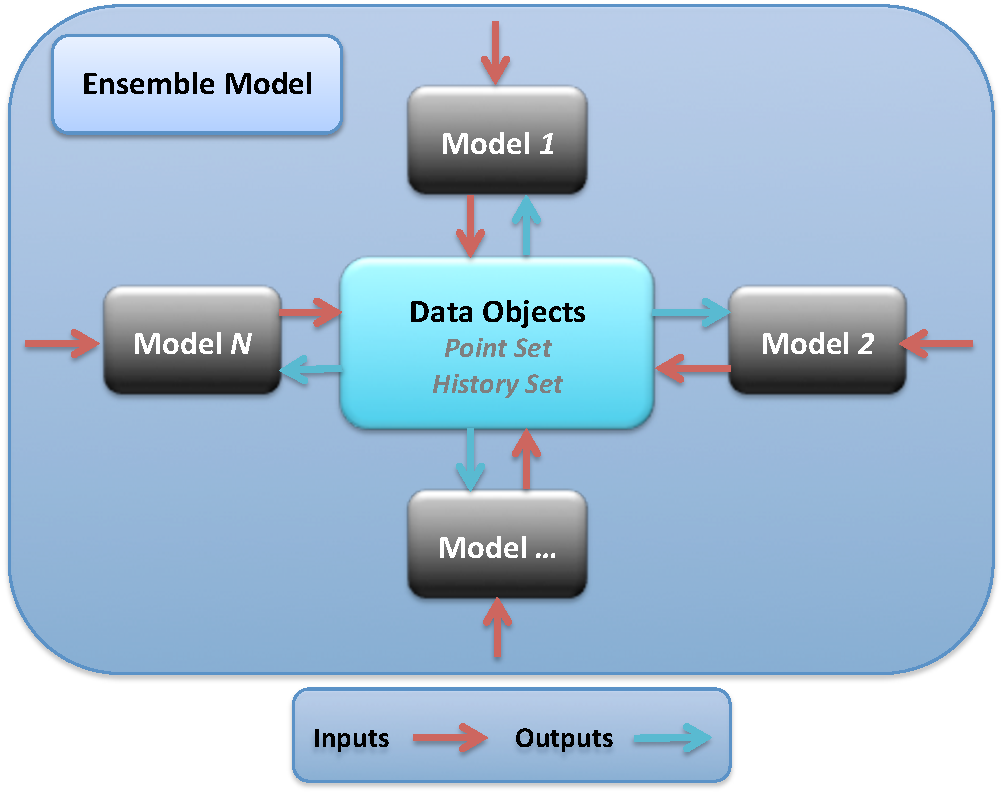
\includegraphics[scale=0.6]{EnsembleModelComunication.pdf}
    \caption{\textit{EnsembleModel} data exchange among sub-models}
    \label{fig:ensembleModelComunication}
\end{figure}

